%!TEX root = ../../../Thesis.tex


\chapter{Compressed Data Structures for Range Searching}


%%%%%%%%%%%%%%%%%%%%%%%%%%%%%%%%%%%%%%%%%%%%%%%%%%%%%%%%%%%%%%%%%%
%%%%%%%%%%%%%%%%%%%%%%%%%%% TITLEPAGE %%%%%%%%%%%%%%%%%%%%%%%%%%%%
%%%%%%%%%%%%%%%%%%%%%%%%%%%%%%%%%%%%%%%%%%%%%%%%%%%%%%%%%%%%%%%%%%
%\newcommand*\samethanks[1][\value{footnote}]{\footnotemark[#1]}

%\title{Compressed Data Structures\\for Range Searching\thanks{Supported by a grant from the Danish National Advanced Technology Foundation.}}
%\author{
%	Philip Bille\thanks{Supported by a grant from the Danish Council for Independent Research $\vert$ Natural Sciences.}
%	\and Inge Li G{\o}rtz\samethanks
% 	\and S{\o}ren Vind
%}
%\date{}
%\institute{DTU Compute, Technical University of Denmark, DK-2800 Kgs. Lyngby, Denmark \\ \email{$\{$phbi,inge,sovi$\}$@dtu.dk}}


%\begin{document}
%\pagestyle{plain}	
%\linenumbers

%\maketitle
%\setcounter{footnote}{0}

% Fix grants, reset footnote counter to arabic.
%\renewcommand{\thefootnote}{\fnsymbol{footnote}}
%\footnotetext[1]{Supported by a grant from the Danish National Advanced Technology Foundation.} %star
%\footnotetext[4]{Supported by a grant from the Danish Council for Independent Research $\vert$ Natural Sciences.} %dagger

%\renewcommand{\thefootnote}{\arabic{footnote}}

%%%%%%%%%%%%%%%%%%%%%%%%%%%%%%%%%%%%%%%%%%%%%%%%%%%%%%%%%%%%%%%%%%
%%%%%%%%%%%%%%%%%%%%%%%%%%% ABSTRACT %%%%%%%%%%%%%%%%%%%%%%%%%%%%%
%%%%%%%%%%%%%%%%%%%%%%%%%%%%%%%%%%%%%%%%%%%%%%%%%%%%%%%%%%%%%%%%%%
\begin{abstract}
We study the orthogonal range searching problem on points that have a significant number of \emph{geometric repetitions}, that is, subsets of points that are identical under translation. Such repetitions occur in scenarios such as image compression, GIS applications and in compactly representing sparse matrices and web graphs. Our contribution is twofold. 
First, we show how to compress geometric repetitions that may appear in standard range searching data structures (such as K-D trees, Quad trees, Range trees, R-trees, Priority R-trees, and K-D-B trees), and how to implement subsequent range queries on the compressed representation with only a constant factor overhead. 
Secondly, we present a compression scheme that efficiently identifies geometric repetitions in point sets, and produces a hierarchical clustering of the point sets, which combined with the first result leads to a compressed representation that supports range searching. 
\end{abstract}

%%%%%%%%%%%%%%%%%%%%%%%%%%%%%%%%%%%%%%%%%%%%%%%%%%%%%%%%%%%%%%%%%%
%%%%%%%%%%%%%%%%%%%%%%%%%% INTRODUCTION %%%%%%%%%%%%%%%%%%%%%%%%%%
%%%%%%%%%%%%%%%%%%%%%%%%%%%%%%%%%%%%%%%%%%%%%%%%%%%%%%%%%%%%%%%%%%
\section{Introduction}
The \emph{orthogonal range searching} problem is to store a set of axis-orthogonal $k$-dimensional objects to efficiently answer \emph{range queries}, such as reporting or counting all objects inside a $k$-dimensional query range. Range searching is a central primitive in a wide range of applications and has been studied extensively over the last 40 years~\cite{bentley1975multidimensional, bentley1979multidimensional, orenstein1982multidimensional, bentley1980decomposable, lueker1978data, lee1980quintary, guttman1984r, clarkson1983fast, kanth1999optimal, van1991dividedk, gaede1998multidimensional, bayer1972organization, arge2008priority, robinson1981kdb, procopiuc2003bkd, comer1979ubiquitous, eppstein2008skip} (Samet presents an overview in \cite{samet1990applications}). 

In this paper we study range searching on points that have a significant number of \emph{geometric repetitions}, that is, subsets of points that are identical under translation. Range searching on points sets with geometric repetitions arise naturally in several scenarios such as data and image analysis \cite{tetko2001pattern, pajarola2000image, dick2009a}, GIS applications \cite{schindler2008detecting, zhu2002efficient, haegler2010a, dick2009a}, and in compactly representing sparse matrices and web graphs~\cite{Galli98compressionof, brisaboa2009k2, brisaboaainterleaved, de2013compact}.

Our contribution is twofold. 
First, we present a simple technique to effectively compress geometric repetitions that may appear in standard range searching data structures (such as K-D trees, Quad trees, Range trees, R-trees, Priority R-trees, and K-D-B trees). Our technique replaces repetitions within the data structures by a single copy, while only incurring an $O(1)$ factor overhead in queries (both in standard RAM model and I/O model of computation). The key idea is to compress the underlying tree representation of the point set into a corresponding minimal DAG that captures the repetitions. We then show how to efficiently simulate range queries directly on this DAG. This construction is the first solution to take advantage of geometric repetitions. Compared to the original range searching data structure the time and space complexity of the compressed version is never worse, and with many repetitions the space can be significantly better. 
Secondly, we present a compression scheme that efficiently identifies translated geometric repetitions. Our compression scheme guarantees that if point set $P_1$ is a translated geometric repetition of point set $P_2$ and $P_1$ and $P_2$ are at least a factor $2$ times their diameter away from other points, the repetition is identified. This compression scheme is based on a hierarchical clustering of the point set that produces a tree of height $O(\log D)$, where $D$ is the diameter of the input point set. Combined with our first result we immediately obtain a compressed representation that supports range searching. 


\subsection{Related Work} 
Several succinct data structures and entropy-based compressed data structures for range searching have recently been proposed, see e.g.,~\cite{makinen2007rank, bose2009succinct, barbay2010compact, farzan2014entropy}. While these significantly improve the space of the classic range searching data structure, they all require at least a $\Omega(N)$ \emph{bits} to encode $N$ points. In contrast, our construction can achieve exponential compression for highly compressible point sets (i.e. where there is a lot of geometric repetitions). 

A number of papers have considered the problem of compactly representing web graphs and tertiary relations~\cite{brisaboa2009k2, brisaboaainterleaved, de2013compact}. They consider how to efficiently represent a binary (or tertiary) quad tree by encoding it as bitstrings. That is, their approach may be considered compact storage of a (sparse) adjacency matrix for a graph. The approach allows compression of quadrants of the quad tree that only contain zeros or ones. However, it does not exploit the possibly high degree of geometric repetition in such adjacency matrices (and any quadrant with different values cannot be compressed).

To the best of our knowledge, the existence of geometric repetitions in the point sets has not been exploited in previous solutions for neither compression nor range searching. Thus, we give a new perspective on those problems when repetitions are present. 

\subsection{Outline}
We first present a general model for range searching, which we call a \emph{canonical range searching data structure}, in Section~\ref{sec:canrsds}. We show how to compress such data structures efficiently and how to support range searching on the compressed data structure in the same asymptotic time as on the uncompressed data structure in Section~\ref{sec:compcrs}. Finally, we present a \emph{similarity clustering} algorithm in Section~\ref{sec:clustering}, guaranteeing that geometric repetitions are clustered such that the resulting canonical range searching data structure is compressible.

%%%%%%%%%%%%%%%%%%%%%%%%%%%%%%%%%%%%%%%%%%%%%%%%%%%%%%%%%%%%%%%%%%
%%%%%%%%%%%%%%%%%%% QUERIES ON COMPRESSED DATA %%%%%%%%%%%%%%%%%%%
%%%%%%%%%%%%%%%%%%%%%%%%%%%%%%%%%%%%%%%%%%%%%%%%%%%%%%%%%%%%%%%%%%

\section{Canonical Range Searching Data Structures}\label{sec:canrsds}
We define a \emph{canonical range searching data structure} $T$, which is an ordered, rooted and labeled tree with $N$ vertices. Each vertex $v \in T$ has an associated $k$-dimensional axis-parallel range, denoted $\range{v}$, and an arbitrary label, denoted $\vlabel(v)$. We let $T(v)$ denote the subtree of $T$ rooted at vertex $v$ and require that ranges of vertices in $T(v)$ are contained in the range of $v$, so for every vertex $u \in T(v)$, $\range{u} \inrange \range{v}$. Leafs may store either points or ranges, and each point or range may be stored in several leafs. The data structure supports \emph{range queries} that produce their result after evaluating the tree through a (partial) traversal starting from the root. In particular, we can only access a node after visiting all ancestors of the node. Queries can use any information from visited vertices. A similar model for showing lower bounds for range searching appeared was used by Kanth and Singh in~\cite{kanth1999optimal}.

Geometrically, the children of a vertex $v$ in a canonical range searching data structure divide the range of $v$ into a number of possibly overlapping ranges. At each level the tree divides the $k$-dimensional regions at the level above into smaller regions. Canonical range searching data structures directly capture most well-known range searching data structures, including Range trees, K-D trees, Quad trees and R-trees as well as B-trees, Priority R-trees and K-D-B trees.


\paragraph{Example: Two-dimensional R tree}
The two-dimensional R tree is a canonical range searching data structure since a vertex covers a range of the plane that contains the ranges of all vertices in its subtree. The range query is a partial traversal of the tree starting from the root, visiting every vertex having a range that intersects the query range and reporting all vertices with their range fully contained in the query range. Figure \ref{fig:r-rep} shows an R tree for a point set, where each vertex is labeled with the range that it covers. The query described for R trees can be used on any canonical range searching data structure, and we will refer to it as a \emph{canonical range query}.

\begin{figure}[tb]
	\begin{center}
	\subfloat[Point Set.]{
		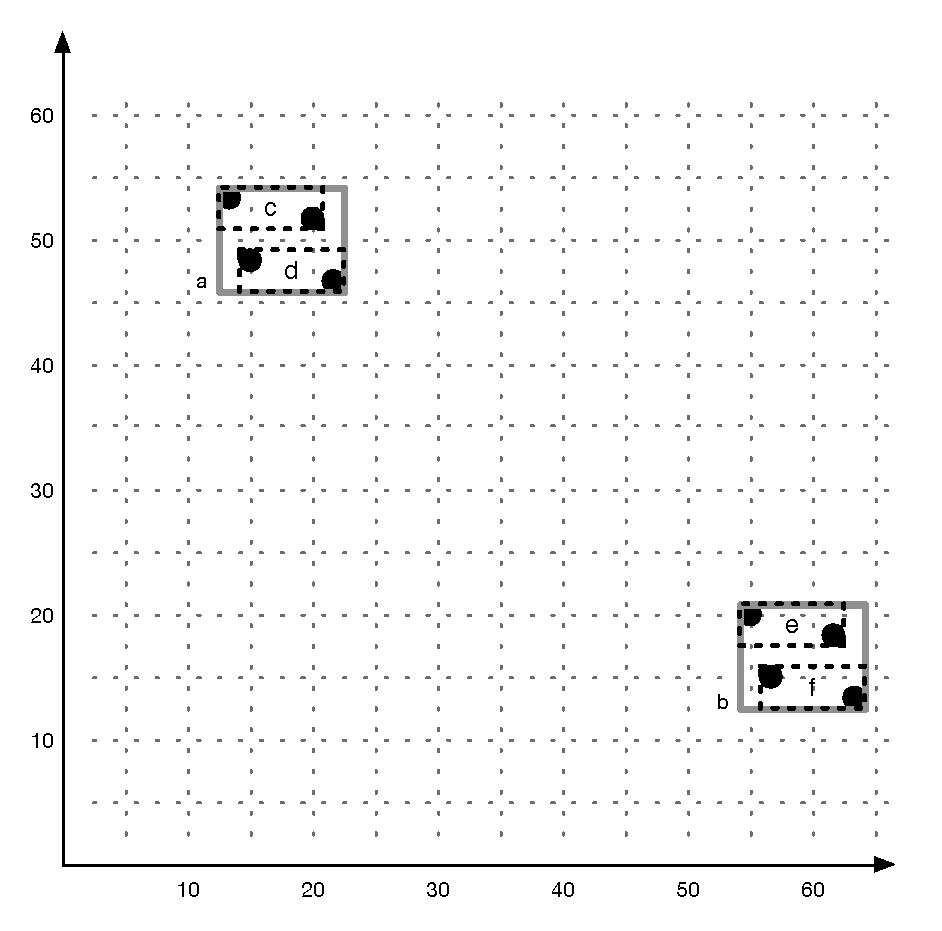
\includegraphics[width=0.4\textwidth]{chapters/papers/compressedrangesearching/r-comp}
	}\quad\quad\quad\quad\subfloat[R tree.]{
		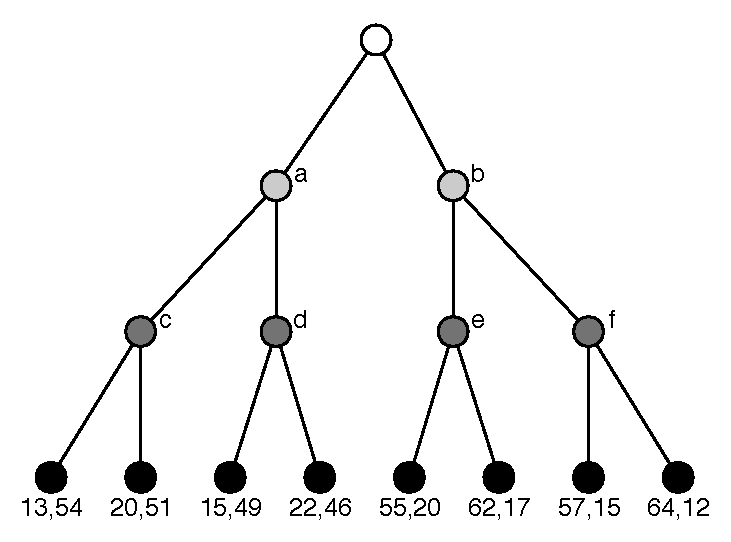
\includegraphics[width=0.4\textwidth]{chapters/papers/compressedrangesearching/rtree-comp}
	}
	\caption{A two-dimensional point set with R tree ranges overlaid, and the resulting R tree. Blue ranges are children of the root in the tree, red ranges are at the second level. A vertex label ($a$ - $h$) in the R tree identifies the range. We have omitted the precise coordinates for the ranges, but e.g. range $a$ spans the range $[13, 22] \times [46, 54]$. \label{fig:r-rep}}
	\end{center}
\end{figure} 

%%%%%%%%%%%%%%%%%%%%%%%%%%%%%%%%%%%%%%%%%%%%%%%%%%%%%%%%%%%%%%%%%%
%%%%%%%%%%%%%%%%%%% ABSOLUTE RANGE TREE TO DAG %%%%%%%%%%%%%%%%%%%
%%%%%%%%%%%%%%%%%%%%%%%%%%%%%%%%%%%%%%%%%%%%%%%%%%%%%%%%%%%%%%%%%%
\section{Compressed Canonical Range Searching}\label{sec:compcrs}
We now show how to compress geometric repetitions in any canonical range searching data structure $T$ while incurring only a constant factor overhead in queries. To do so we convert $T$ into a \emph{relative tree} representation, which we then compress into a minimal DAG representation that replaces geometric repetitions by single occurrences. We then show how to simulate a range query on $T$ with only constant overhead directly on the compressed representation. Finally, we extend the result to the I/O model of computation.

\subsection{The Relative Tree}
A \emph{relative tree} $R$ is an ordered, rooted and labeled tree storing a relative representation of a canonical range searching data structure $T$. The key idea is we can encode a range or a point $r = [ x_1, x'_1 ] \times \ldots \times [ x_k, x'_k ]$ as two $k$-dimensional vectors $\position(r) = (x_1, \ldots, x_k)$ and $\rangespan(r) = (x'_1 - x_1, \ldots, x'_k - x'_k)$ corresponding to an \emph{origin position} and an \emph{extent} of $r$. We use this representation in the relative tree, but only store extent vectors at vertices explicitly. The origin position vector for the range $\range{v}$ of a vertex $v \in R$ is calculated from offset vectors stored on the path from the root of $R$ to $v$, denoted $\rootpath(v)$. 

Formally, each vertex $v \in R$ stores a label, $\vlabel(v)$, and a $k$-dimensional extent vector $\rangespan(\range{v})$. Furthermore, each edge $(u, v) \in R$ stores an offset vector $\offset(u, v)$. The position vector for $\range{v}$ is calculated as $\position(\range{v}) = \sum_{(a, b) \in \rootpath(v)} \offset(a, b)$.
We say that two vertices $v, w \in R$ are \emph{equivalent} if the subtrees rooted at the vertices are isomorphic, including all labels and vectors. That is, $v$ and $w$ are equivalent if the two subtrees $R(v)$ and $R(w)$ are equal. 

It is straightforward to convert a canonical range searching data structure into the corresponding relative tree.
\begin{lemma}\label{lem:abs2rel}
Given any canonical range searching data structure $T$, we can construct the corresponding relative tree $R$ in linear time and space. 
\end{lemma}
\begin{proof}
First, note that a relative tree allows each vertex to store extent vectors and labels. Thus, to construct a relative tree $R$ representing the canonical range searching data structure $T$, we can simply copy the entire tree including extent vectors and vertex labels. So we only need to show how to store offset vectors in $R$ to ensure that the ranges for each pair of copied vertices are equal.

Consider a vertex $v \in T$ and its copy $v_R \in R$ and their parents $w \in T$ and $w_R \in R$. Since the extent vector and vertex labels are copied, $\rangespan(\range{v}) = \rangespan(\range{v_R})$ and $\vlabel(v) = \vlabel(v_R)$. The offset vector for the $(w_R, v_R)$ edge is $\offset(w_R, v_R) = \position(\range{v}) - \position(\range{w})$. We assume the offset for the root is the 0-vector. Observe that summing up all the offset vectors on $\rootpath(v)$ is exactly $\position(\range{v})$, and so $\position(\range{v_R}) = \position(\range{v})$.

Since each vertex and edge in $T$ is only visited a constant number of times during the mapping, the construction time for $R$ is $O(N)$. The total number of labels stored by $R$ is asymptotically equal to the number of labels stored by $T$. Finally, the degrees of vertices does not change from $T$ to $R$. Thus, if $v \in T$ is mapped to $v_R \in R$ and $v$ requires $s$ space, $v_R$ requires $\Theta(s)$ space.
\end{proof}

\subsection{The Data Structure}
The compressed canonical data structure is the minimal DAG $G$ of the relative tree $R$ for $T$. By Lemma~\ref{lem:abs2rel} and~\cite{downey1980variations} we can build it in $O(N)$ time. Since $G$ replaces equivalent subtrees in $R$ by a single subtree, geometric repetitions in $T$ are stored only once in $G$. For an example, see Figure~\ref{fig:r-compression}. 
\begin{figure}[tb]
	\begin{center}
	\subfloat[Relative tree.]{
		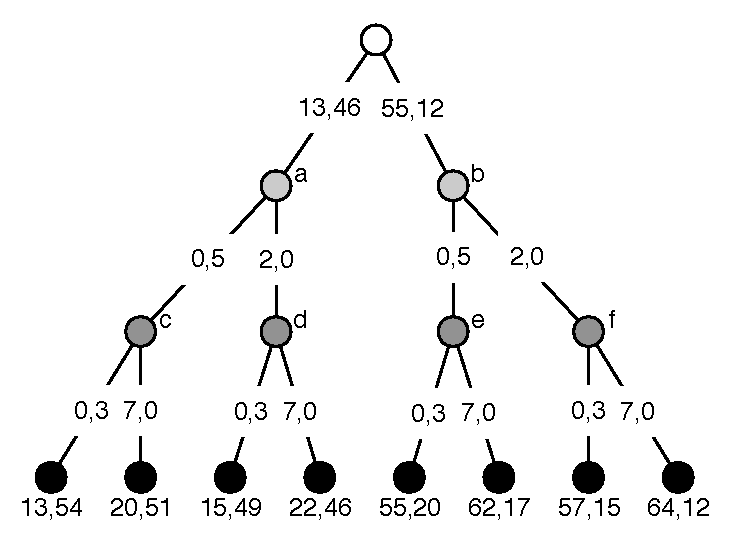
\includegraphics[width=0.4\textwidth]{chapters/papers/compressedrangesearching/rtree-relative}
	}\quad\quad\quad\quad\subfloat[Minimal DAG.]{
		\makebox[0.4\textwidth]{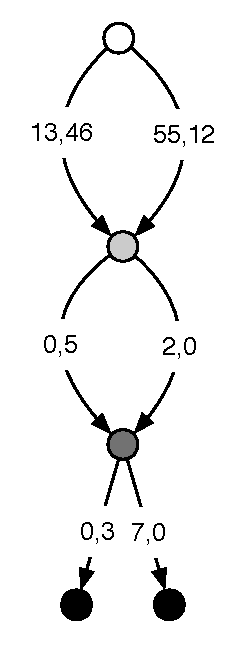
\includegraphics[height=0.3\textwidth]{chapters/papers/compressedrangesearching/rtree-dag}}
	}
	\caption{The relative tree obtained from the R tree from Figure \ref{fig:r-rep} and the resulting minimal DAG $G$ generating the tree. Only coordinates of the lower left corner of the ranges in the R tree are shown. In the relative tree, the absolute coordinates for the points are only shown for illustration, in order to see that the relative coordinates sum to the absolute coordinate along the root-to-leaf paths. \label{fig:r-compression}}
	\end{center}
\end{figure}

Now consider a range query $Q$ on the canonical range searching data structure $T$. We show how to simulate $Q$ efficiently on $G$. Assuming $v_G \in G$ generates $v_R \in R$, we say that $v_G$ generates $v \in T$ if $v_R$ is the relative tree representation of $v$. When we visit a vertex $v_G \in G$, we calculate the origin position $\position(\range{v_G})$ from the sum of the offset vectors along the root-to-$v_G$ path. The origin position for each vertex can be stored on the way down in $G$, since we may only visit a vertex after visiting all ancestors (meaning that we can only arrive at $v_G$ from a root-to-$v_G$ path in $G$). Thus, it takes constant time to maintain the origin position for each visited vertex. Finally, a visit to a child of $v \in T$ can be simulated in constant additional time by visiting a child of $v_G \in G$. So we can simulate a visit to $v \in T$ by visiting the vertex $v_G \in G$ that generates $v$ and in constant time calculate the origin position for $v_G$. 

Any label comparison takes the same time on $G$ and $T$ since the label must be equal for $v_G \in G$ to generate $v \in T$. Now, since there is only constant overhead in visiting a vertex and comparing labels, it follows that if $Q$ uses $t$ time we can simulate it in $O(t)$ time on $G$. In summary, we have the following result.

\begin{theorem}\label{thm:compCan}
	Given a canonical range searching data structure $T$ with $N$ vertices, we can build the minimal DAG representation $G$ of $T$ in linear time. The space required by $G$ is $O(n)$, where $n$ is the size of the minimal DAG for a relative representation of $T$. We can support any query $Q$ on $T$ that takes time $t$ on $G$ in time $O(t)$. 
\end{theorem} 
As an immediate corollary, we get the following result for a number of concrete range searching data structures.
\begin{corollary}
	Given a K-D tree, Quad tree, R tree or Range tree, we can in linear time compress it into a data structure using space proportional to the size of the minimal relative DAG representation which supports canonical range searching queries with $O(1)$ overhead.
\end{corollary}


%%%%%%%%%%%%%%%%%%%%%%%%%%%%%%%%%%%%%%%%%%%%%%%%%%%%%%%%%%%%%%%%%%
%%%%%%%%%%%%%%%%%%%%%% I/O EFFICIENT QUERIES %%%%%%%%%%%%%%%%%%%%%
%%%%%%%%%%%%%%%%%%%%%%%%%%%%%%%%%%%%%%%%%%%%%%%%%%%%%%%%%%%%%%%%%%
\subsection{Extension to the I/O Model}
We now show that Theorem~\ref{thm:compCan} extends to the I/O model of computation. We assume that each vertex in $T$ require $\Theta(B)$ space, where $B$ is the size of a disk block. To allow for such vertices, we relax the definition of a canonical range searching data structure to allow it to store $B$ $k$-dimensional ranges. From Lemma~\ref{lem:abs2rel} and~\cite{downey1980variations}, if a vertex $v \in T$ require $\Theta(B)$ space, then so does the corresponding vertex $v_G \in G$. Thus, the layout of the vertices on disk does not asymptotically influence the number of disk reads necessary to answer a query, since only a constant number of vertices can be retrieved by each disk read. This means that visiting a vertex in either case takes a constant number of disk blocks, and so the compressed representation does not asymptotically increase the number of I/Os necessary to answer the query. Hence, we can support any query $Q$ that uses $p$ I/Os on $T$ using $O(p)$ I/Os on $G$. 


%%%%%%%%%%%%%%%%%%%%%%%%%%%%%%%%%%%%%%%%%%%%%%%%%%%%%%%%%%%%%%%%%%
%%%%%%%%%%%%%%%%%%%%% SIMILARITY CLUSTERING %%%%%%%%%%%%%%%%%%%%%%
%%%%%%%%%%%%%%%%%%%%%%%%%%%%%%%%%%%%%%%%%%%%%%%%%%%%%%%%%%%%%%%%%%
\section{Similarity Clustering}\label{sec:clustering}
We now introduce the \emph{similarity clustering} algorithm. Even if there are significant geometric repetitions in the point set $P$, the standard range searching data structures may not be able to capture this and may produce data structures that are not compressible. The similarity clustering algorithm allows us to create a canonical range searching data structure for which we can guarantee good compression using Theorem~\ref{thm:compCan}.

\subsection{Definitions}
\paragraph{Points and point sets}
We consider points in $k$-dimensional space, assuming $k$ is constant. The distance between two points $p_1$ and $p_2$, denoted $d(p_1, p_2)$, is their euclidian distance. We denote by $P = \{ p_1, p_2, \ldots, p_r \}$ a point set containing $r$ points. We say that two point sets $P_1, P_2$ are \emph{equivalent} if $P_2$ can be obtained from $P_1$ by translating all points with a constant $k$-dimensional offset vector.

The minimum distance between a point $p_q$ and a point set $P$, $\mindist(P, p_q) = \min_{p \in P} d(p, p_q)$, is the distance between $p_q$ and the closest point in $P$. The minimum distance between two point sets $P_1, P_2$ is the distance between the two closest points in the two sets, $\mindist(P_1, P_2) = \min_{p_1 \in P_1, p_2 \in P_2} d(p_1, p_2)$. These definitions extend to maximum distance in the natural way, denoted $\maxdist(P, p_q)$ and $\maxdist(P_1, P_2)$. The diameter of a point set $P$ is the maximum distance between any two points in $P$, $\diameter(P) = \max_{p_1, p_2 \in P} d(p_1, p_2) = \maxdist(P, P)$.

A point set $P_1 \subset P$ is \emph{lonely} if the distance from $P_1$ to any other point is more than twice $\diameter(P_1)$, i.e. $\mindist(P_1, P \setminus P_1) > 2 \times \diameter(P_1)$.

\paragraph{Clustering}
A hierarchical clustering of a point set $P$ is a tree, denoted $\clustering(P)$, containing the points in $P$ at the leaves. Each node in the tree $\clustering(P)$ is a cluster containing all the points in the leaves of its subtree. The root of $\clustering(P)$ is the cluster containing all points. We denote by $\points(v)$ the points in cluster node $v \in \clustering(P)$. Two cluster nodes $v, w \in \clustering(P)$ are equivalent if $\points(v)$ is equivalent to $\points(w)$ and if the subtrees rooted at the nodes are isomorphic such that each isomorphic pair of nodes are equivalent.

\subsection{Hierarchical Clustering Algorithm for Lonely Point Sets}
Order $P$ in lexicographically increasing order according to their coordinates in each dimension, and let $\Delta(P)$ denote the ordering of $P$.
The similarity clustering algorithm performs a greedy clustering of the points in $P$ in levels $i = 0, 1, \ldots, \log D+1$, where $D = \diameter(P)$. Each level $i$ has an associated clustering distance threshold $d_i$, defined as $d_0 = 0$ and $d_i = 2^{i-1}$ for all other $i$.

The clustering algorithm proceeds as follows, processing the points in order $\Delta(P)$ at each level. If a point $p$ is not clustered at level $i > 0$, create a new cluster $C_i$ centered around the point $p$ (and its cluster $C_{i-1}$ at the previous level). Include a cluster $C_{i-1}$ from level $i-1$ in $C_i$ if $\maxdist(\points(C_{i-1}), p) \leq d_i$. The clusters at level $0$ contain individual points and the cluster at level $\log D+1$ contains all points.

\begin{lemma}\label{lem:clustAlg}
	Given a set of points $P$, the similarity clustering algorithm produces a clustering tree containing equivalent clusters for any pair of equivalent lonely point sets.
\end{lemma}
\begin{proof}
Let $P_1$ and $P_2$ be two lonely point sets in $P$ such that $P_1$ and $P_2$ are equivalent, and let $d = \diameter(P_1) = \diameter(P_2)$. Observe that a cluster formed at level $i$ has at most diameter $2d_i = 2^i$. Thus, since all points are clustered at every level and all points outside $P_1$ have a distance greater than $2d$ to any point in $P_1$, there is a cluster $c \in \clustering(P)$ formed around point $a \in P_1$ at level $j = \lceil \log d \rceil$ containing no points outside $P_1$. Now, assume some point $p \in P_1$ is not in $\points(c)$. As all unclustered points within distance $2^j \geq d$ from $a$ are included in $c$, this would mean that $p$ was clustered prior to creating $c$. This contradicts the assumption that $P_1$ is lonely, since it can only happen if some point outside $P_1$ is closer than $2d$ to $p$. Concluding, $c$ contains exactly the points in $P_1$. The same argument naturally extends to $P_2$.

Now, let $C_1, C_2$ be the clusters containing the points from $P_1, P_2$, respectively. Observe that $\points(C_1)$ and $\points(C_2)$ are equivalent. Furthermore, because each newly created cluster process candidate clusters to include in the same order, the resulting trees for $C_1$ and $C_2$ are isomorphic and have the same ordering. Thus, the clusters $C_1$ and $C_2$ are equivalent.
\end{proof}

Because the clustering proceeds in $O(\log D)$ levels, the height of the clustering tree is $O(\log D)$. Furthermore, by considering all points and all of their candidates at each level, the clustering can be implemented in time $O(N^2 \log D)$. Observe that the algorithm allows creation of paths of clusters with only a single child cluster. If such paths are contracted to a single node to reduce the space usage, the space required is $O(N)$ words. In summary, we have the following result. 

\begin{theorem}\label{thm:clustering}
	Given a set of $N$ points with diameter $D$, the similarity clustering algorithm can in $O(N^2 \log D)$ time create a tree representing the clustering of height $O(\log D)$ requiring $O(N)$ words of space. The algorithm guarantees that any pair of equivalent lonely point sets results in the same clustering, producing equivalent subtrees in the tree representing the clustering.
\end{theorem}

Since the algorithm produces equivalent subtrees in the tree for equivalent lonely point sets, the theorem gives a compressible canonical range searching data structure for point sets with many geometric repetitions.


\section{Open Problems}
The technique described in this paper for generating the relative tree edge labels only allows for translation of the point sets in the underlying subtrees. However, the given searching technique and data structure generalizes to scaling and rotation (if simply storing a parent-relative scaling factor and rotation angle in each node, along with the nodes parent-relative translation vector). We consider it an open problem to efficiently construct a relative tree that uses such transformations of the point set. 

Another interesting research direction is if it is possible to allow for small amounts of noise in the point sets. That is, can we represent point sets that are almost equal (where few points have been moved a little) in a compressed way? An even more general question is how well one can do when it comes to compression of higher dimensional data in general.

Finally, the $O(N^2 \log D)$ time bound for generating the similarity clustering is prohibitive for large point sets. So an improved construction would greatly benefit the possible applications of the clustering method and is of great interest.

%\bibliographystyle{splncs03}

%\nocite{*}
%\bibliography{references}

%\end{document}
